\documentclass[a4paper,12pt,UTF8]{article}
\usepackage{CTEX}
\usepackage{graphicx}
\usepackage{diagbox}
\usepackage{tikz}
\usepackage{setspace}
\usepackage{subfigure}
\usepackage{indentfirst}
\usepackage{listings}
\usepackage{xcolor}

\lstset{
    basicstyle=\tt,
    %行号
    numbers=left,
    rulesepcolor=\color{red!20!green!20!blue!20},
    %escapeinside=``,
    %xleftmargin=0em,xrightmargin=5em, aboveskip=5em,
    %背景框
    framexleftmargin=1.5mm,
    frame=shadowbox,
    %背景色
    backgroundcolor=\color[RGB]{245,245,244},
    %样式
    keywordstyle=\color{blue}\bfseries,
    identifierstyle=\bf,
    numberstyle=\color[RGB]{0,192,192},
    commentstyle=\it\color[RGB]{96,96,96},
    stringstyle=\rmfamily\slshape\color[RGB]{128,0,0},
    %显示空格
    showstringspaces=false
}
\begin{document}
    \begin{spacing}{2.0}
        \title{\textbf{\huge{人工智能课程设计实验报告}}}
        \date{}
        \maketitle
        \begin{figure}[h]
            \centering
        
\includegraphics[width=7cm,height=7cm]{tongji_logo}
        \end{figure}
    \end{spacing}   
    {
    \Large
        \textbf{
        \begin{flushleft}
        学\hspace{1cm}号:\hspace{4cm}2151769\\
        姓\hspace{1cm}名:\hspace{4cm}吕博文\\
        专\hspace{1cm}业:\hspace{3cm}计算机科学与技术\\
        授课老师:\hspace{4cm}王俊丽\\
        \end{flushleft}
        }
    }
\newpage
\begin{flushleft}
{
       \Large{
        \textbf{一、问题概述\\}
       }
       \large{
        \hspace{1cm}\textbf{1、问题描述\\}
       }
       \hspace{1cm}\normalsize{
            本次人工智能实验project1是基于搜索专题的一次练习,主要包含内容有:无信息搜索和有信息
            搜索,project1基于吃豆人这样一个简单的游戏,要求我们编些算法实现各种搜索策略:深度优先搜索(dfs)、
            宽度优先搜索(bfs),一致代价搜索(ucs),A*搜索等算法;特别地对于比较重要的A*算法,该项目在最后几个
            子任务要求我们去编写适合题目的启发式函数,同时本项目事先提供了比较多的基础代码,在python的基础上
            广泛使用了class类定义来解决问题的方式,要求同学们对python中类的知识有一定的了解方便之后算法的编写,
            项目还额外提供了界面展示的许多代码,使得最终的结果可以实现简单的可视化,也一定程度上增加了该项目的趣味性。\\

    }
    \large{
        \hspace{1cm}\textbf{2、项目已有代码阅读与理解\\}
    }
    \hspace{1cm}\normalsize{
        本项目提供了许多预先的代码,其中重点需要我们阅读和理解的主要有以下五个文件:\\
        \hspace{1cm}$(1)seach.py:$是写主要搜索算法的文件,在该文件中需要我们完成dfs,bfs,ucs以及A*
        搜索算法的python实现。\\
        \hspace{1cm}$(2)searchAgents.py:$该文件主要包括控制智能体在迷宫中移动的各种类的实现,包括最基本的
        searchAgent用来控制智能体基础的移动,以及存储智能体移动的相关信息,如何得到该状态下的后继状态等函数,
        也包括许多针对不同的问题所编写出的类,比如PositionSearch problem类用来寻找迷宫中的某一位置,CornerProblem
        类用来寻找最快的到达迷宫四个角落的算法,同时也是需要我们自己实现的一个类,最后还有foodSearch problem类用来寻找迷宫中的所有
        食物的一个类,同时这里面还包含了需要我们自己编写的启发式函数等等。\\
        \hspace{1cm}$(3)util.py$该文件是项目本身提供的一些比较实用的数据结构封装类,在编写search.py中的各种算法时
        合理利用这些类可以提高代码编写效率。\\
        \hspace{1cm}$(4)game.py:$该文件是整个项目得以运行的整个逻辑代码,其中包括了整个游戏的所有信息的存储,方向点位的确定,食物位置,智能体位置
        的确定,迷宫的构建,整个项目运行过程中智能体所需要存储的信息。\\
        \hspace{1cm}$(5)Pacman.py:$整个项目运行的主文件,调用各种其他py文件封装好的模块,驱动整个项目的运行。\\

        
    }
    \large{
        \hspace{1cm}\textbf{3、解决问题思路与方法\\}
    }
    \normalsize{
        \hspace{1cm}综合整个问题框架来看,本项目主要考察了一些经典搜索算法在人工智能领域的实现,同时不同于常规算法编写的是,
        本项目给出了庞大的已有的项目代码,将许多零散的信息封装成类统一处理,要求我们在理解算法知识的同时还要能够初步
        理解本项目中的一些类的定义,类成员的调用,类函数的调用等等,因为在主要搜索算法的编写中,函数传入的参数是固定的
        ,所以我们必须结合类中可以使用的一些成员函数来实现整个算法。\\
        \hspace{1cm}首先考虑$search.py$文件中各种算法的编写,考虑到项目本身也给出了提示,所以我打算使用$util.py$中定义
        好的许多数据结构来帮助解决算法的编写,初步想法是:$dfs$用到栈,$bfs$用到队列,$ucs$与$A*$算法用到优先队列等等。\\
        \hspace{1cm}考虑$searchAgents.py$中对一些类函数的补全时,我们可以参考项目中已有的代码规范与格式,对这些类函数做出
        符合实际问题要求的补全,同样,对于启发式函数的编写,可以考虑先在草稿纸上写出几种可行的方案,然后一个个试验,取最优的
        启发式函数作为最终解。\\
    }
    \Large{
        \textbf{
            二、算法设计\\
        }
    }
    \large{
        \hspace{1cm}\textbf{1、$dfs$算法:\\}
    }
    \normalsize{
        \hspace{1cm}$dfs$算法是深度优先搜索算法的简称,对于深度优先搜索我们首选用递归函数实现,但因为
        本题对函数参数已经加以限制,所以我们考虑递归函数的根本在于程序栈的调用,所以我们使用栈这个数据结构
        去模拟递归函数的调用来实现dfs的完成。\\
        \hspace{1cm}我们定义栈$st$,栈中元素分为两部分,一部分是当前状态的坐标,另一部分是从起点到该状态点
        所走过的路径(用具体每次向哪个方向走代替),然后我们可以定义一个集合$visited$来记录当前状态坐标是否
        访问过,循环终止条件为栈空,每次循环首先去除栈顶元素并判断是否到达终点,如果到达,直接返回路径$path$,
        反之,遍历找到该状态的所有可能后继节点,把那些没有访问过的压入栈中继续下一次循环。\\
    }
    \large{
        \hspace{1cm}\textbf{2、$bfs$算法:\\}
    }
    \normalsize{
        \hspace{1cm}$bfs$算法是宽度优先搜索算法的简称,对于$bfs$我们考虑使用队列来实现,代码基本架构和$dfs$相似
        ,只是把栈换成了队列,基于队列先进先出的性质,$bfs$算法总能每次遍历一层节点,逐步扩展,最终找到解。\\
    }
    \large{
        \hspace{1cm}\textbf{3、$ucs$算法:\\}
    }
    \normalsize{
        \hspace{1cm}$ucs$算法是一致代价搜索算法的简称,在算法领域的实现和$Dijstra$算法相似,与$bfs$每次
        直接扩展当前节点的所有相邻后继节点不同,$ucs$则是优先扩展距离起点最近的点的后继,并且由于贪心思想,
        这样的每次扩展最后找到的一定是最短路径,所以在实现$ucs$算法时我们需要使用优先队列,并以当前节点到
        起点的距离作为优先比较键值,其他代码实现上与$bfs$类似。\\
    }
    \large{
        \hspace{1cm}\textbf{4、$A*$算法:\\}
    }
    \normalsize{
        \hspace{1cm}$A*$算法是在$ucs$算法基础上的改进,它同样使用优先队列扩展临近节点,但$A*$算法定义了启发式
        函数的定义,也即是当前扩展节点的优先级不仅考虑节点与起始点的实际距离同时还要考虑当前节点到终点的估计距离,
        而这个估计距离由启发式函数确定,特别地,如果启发式函数始终返回零,那么此时$A*$算法实际上就是$ucs$算法。\\
    }
    \large{
        \hspace{1cm}\textbf{5、$cornerProblem$类设计:\\}
    }
    \normalsize{
        \hspace{1cm}在解决$cornerProblem$类设计时,问题要求我们设计寻找迷宫四个角落的算法实现类,所以我们考虑改变每个
        状态下记录的值,不仅记录当前节点坐标,同时记录当前状态已经访问过的角落坐标,当且仅当当前状态下访问过的角落数量为
        4时判断为结束状态。\\
    }
    \large{
        \hspace{1cm}\textbf{6、$cornersHeuristic$启发式函数设计:\\}
    }
    \normalsize{
        \hspace{1cm}在针对$cornersHeuristic$问题设计启发式函数时,我们定义在每次当前节点查看到还未访问过的节点的实际距离,
        我们取这些距离的最大值显然可以证明,这个值一定是实际值的一个下界且满足一致性的要求,可以作为启发式函数,在实际解决该
        问题的时候我还尝试了使用其他的启发式函数比如用曼哈顿距离来估算最大值作为估计值,或者以直线距离来估计距离,最后还是选择
        了当前的算法,因为其在结果表现上显得最优。\\
    }
    \large{
        \hspace{1cm}\textbf{7、$foodHeuristic$启发式函数设计:\\}
    }
    \normalsize{
        \hspace{1cm}在设计$foodHeuristic$的启发式函数时,我们的思路和$cornersHeuristic$类似,都是在当前节点查看还未访问
        过的节点的实际距离取这些距离的最大值,只不过这时候目标位置不仅仅只是四个角落,是题目中指定的位置,这里有一个小技巧,
        我们可以在类的构造函数处定义一个字典来记录每次一个坐标到对应food位置的距离,这样就可以防止重复计算,加快计算效率。\\
    }
    \large{
        \hspace{1cm}\textbf{8、$ClosestDotSearchAgent$设计:\\}
    }
    \normalsize{
        \hspace{1cm}这里在寻找距离当前位置最近的一个food位置时,我们只需要调用之前编写好的$ucs$函数即可。\\
    }
    \Large{
        \textbf{
            三、算法实现\\
        }
    }
    \large{
        \hspace{1cm}\textbf{1、$dfs$算法:\\}
    }
    \normalsize{
        \hspace{1cm}核心代码如下:\\
    }
    \scriptsize{
        \begin{lstlisting}
st=util.Stack() #定义栈
start_pos=[problem.getStartState(),[]] #栈内元素为坐标和起始点到该点的路径
st.push(start_pos)
visited=set()#记录当前坐标是否访问过,防止重复访问
while not st.isEmpty():
    [now_pos,path]=st.pop()#取出栈顶元素
    if(problem.isGoalState(now_pos)):
        return path #如果已经到达目标地点,直接返回path路径
    if not now_pos in visited:
        visited.add(now_pos)#将该节点标记为已读
        for new_state,new_action,new_cost in problem.getSuccessors(now_pos):
            #遍历新节点
            new_path=path+[new_action]
            st.push([new_state,new_path])
util.raiseNotDefined()
        \end{lstlisting}
    }
    \normalsize{
        \hspace{1cm}和算法思想里讲述的实现方式大致类似,通过调用栈这个数据结构
        模拟函数递归的过程,通过类自定义的函数$problem.getStartState()$得到初始状态,
        $problem.isGoalState()$判断是否到达终点,$ problem.getSuccessors()$得到当前状态
        的下一状态,最后返回$path$。\\
    }
    \large{
        \hspace{1cm}\textbf{2、$bfs$算法:\\}
    }
    \normalsize{
        \hspace{1cm}核心代码如下:\\
    }
    \scriptsize{
        \begin{lstlisting}
#bfs代码和dfs代码逻辑相似,主要是把栈换成了队列
q=util.Queue()#定义队列
start_pos=[problem.getStartState(),[]] #栈内元素为坐标和起始点到该点的路径
q.push(start_pos)
visited=set()
while not q.isEmpty():
    [now_pos,path]=q.pop()
    if(problem.isGoalState(now_pos)):
        return path
    if not now_pos in visited:
        visited.add(now_pos)
        for new_state,new_action,new_cost in problem.getSuccessors(now_pos):
            new_path=path+[new_action]
            q.push([new_state,new_path])
util.raiseNotDefined()
        \end{lstlisting}
    }
    \normalsize{
        \hspace{1cm}$bfs$算法的实现等同于$dfs$,将数据结构从栈换为了队列,其他变化不大。\\
    }
    \large{
        \hspace{1cm}\textbf{3、$ucs$算法:\\}
    }
    \normalsize{
        \hspace{1cm}核心代码如下:\\
    }
    \scriptsize{
        \begin{lstlisting}
#UCS是一致代价搜索,在算法领域实质上等价与Dijstra算法,我们在实现该算法时采用
#优先队列的数据结构,并按照距离起始点的距离作为优先比较的键值,值越小,优先级越高
pq=util.PriorityQueue()#定义优先队列
start_pos=problem.getStartState()
distance={start_pos:0}
#distance字典刻画了图中的每个点距离起始点的最短路径长度,没有加入字典时默认为无限大
visited=set()#标记该位置是否访问过
pq.push([start_pos,[]],distance[start_pos])
while not pq.isEmpty():
    [now_pos,now_path]=pq.pop()
    if now_pos in visited:
        continue
    visited.add(now_pos)
    if problem.isGoalState(now_pos):
        return now_path
    for new_pos,new_action,step_cost in problem.getSuccessors(now_pos):
        new_cost=step_cost+distance[now_pos]
        if not new_pos in distance or new_cost < distance[new_pos]:
            distance[new_pos]=new_cost
            new_path=now_path+[new_action]
            pq.push([new_pos,new_path],distance[new_pos])
util.raiseNotDefined()
        \end{lstlisting}
    }
    \normalsize{
        \hspace{1cm}在$ucs$算法中我们将数据结构换为优先队列,所以我们额外定义
        了一个字典变量$distance$用来记录当前节点距离起始点的距离,并以该距离作为
        优先队列排序的关键词插入优先队列中,其他方面的实现和$bfs$类似。\\
    }
    \large{
        \hspace{1cm}\textbf{4、$A*$算法:\\}
    }
    \normalsize{
        \hspace{1cm}核心代码如下:\\
    }
    \scriptsize{
        \begin{lstlisting}
#A*搜索是对UCS搜索和贪婪代价搜索的合理结合,其主要思想和UCS算法相似,
#关键在于启发式函数的构造
visited=set()
pq=util.PriorityQueue()
start_pos=problem.getStartState()
start_state=[start_pos,[]]
f_score={start_pos:heuristic(start_pos,problem)}
g_score={start_pos:0}
pq.push(start_state,f_score[start_pos])
while not pq.isEmpty():
    [now_pos,now_path]=pq.pop()
    if now_pos in visited:
        continue
    visited.add(now_pos)
    if problem.isGoalState(now_pos):
        return now_path
    for new_pos,new_action,step_cost in problem.getSuccessors(now_pos):
        new_cost=step_cost+g_score[now_pos]
        if not new_pos in g_score or new_cost<g_score[new_pos]:
            g_score[new_pos]=new_cost
            f_score[new_pos]=g_score[new_pos]+heuristic(new_pos,problem)
            new_path=now_path+[new_action]
            pq.push([new_pos,new_path],f_score[new_pos])

util.raiseNotDefined()
        \end{lstlisting}
    }
    \normalsize{
        \hspace{1cm}$A*$算法中的关键在于启发式函数的编写,$A*$算法本身的实现$ucs$类似,
        只不过这时候我们是以启发式函数$f(n)=g(n)+h(n)$的值作为优先队列排序的关键元素,
        这个公式中$g(n)$就是前面$ucs$算法中的当前节点距离起始点的距离,而$h(n)$则是当前
        节点到目标节点的估计距离,是启发式函数的返回值,在这里我们调用了启发式函数$heuristic$,
        具体实现在启发式函数内部实现。\\
    }
    \large{
        \hspace{1cm}\textbf{5、$cornerProblem$类设计:\\}
    }
    \normalsize{
        \hspace{1cm}核心代码如下:\\
    }
    \hspace{1cm}\normalsize{1、类的构造函数中的补充内容:\\}
    \scriptsize{
        \begin{lstlisting}
"*** YOUR CODE HERE ***"
self.startingGameState=startingGameState 
#将父类的gamestate记录到子类
self.HeuristicInfo={}
#该字典表示在搜索过程中记录下的有效信息,防止多次查找同一信息,降低效率
        \end{lstlisting}                   
    }
    \hspace{1cm}\normalsize{2、类的初始状态返回函数中的补充内容:\\}
    \scriptsize{
        \begin{lstlisting}
state=(self.startingPosition,())
#一个代表xy坐标,一个代表当前状态下已经访问过的corner的集合
return state
        \end{lstlisting}
    }
    \hspace{1cm}\normalsize{3、类的后继状态返回函数中的补充内容:\\}
    \scriptsize{            
        \begin{lstlisting}
    "*** YOUR CODE HERE ***"
x,y = state[0]
dx, dy = Actions.directionToVector(action)
nextx, nexty = int(x + dx), int(y + dy)
hitsWall = self.walls[nextx][nexty]
if not hitsWall:
    new_state=((nextx,nexty),state[1])
    if (nextx,nexty) in self.corners: 
        if not (nextx,nexty) in state[1]:
            new_state=((nextx,nexty),(state[1]+((nextx,nexty),)))
#(state[1]+((nextx,nexty),))是一个新的元组构造方法,因为元组无法直接加减元素
    successors.append((new_state,action,1))
        \end{lstlisting}
    }
    \normalsize{
        \hspace{1cm}在解决$cornerproblem$问题中,我们主要是改变了当前状态的定义,除了存储当前位置坐标,
        还存储了当前已经访问过的角落坐标,这样对于解决这种多目标搜索的问题比较有利,与此同时,后继状态返回
        函数也需要按需做出相应的改变。\\
    }
    \large{
        \hspace{1cm}\textbf{6、$cornersHeuristic$启发式函数设计:\\}
    }
    \normalsize{
        \hspace{1cm}核心代码如下:\\
    }
    \scriptsize{
        \begin{lstlisting}
#我们设计启发式函数的思路是,在每次当前节点查看到还未访问过的节点的实际距离,
#我们取这些距离的最大值
#显然可以证明,这个值一定是实际值的一个下界且满足一致性的要求,可以作为启发式函数
(now_x,now_y)=state[0]
visited_corners=set(state[1])
all_corners=set(corners)
unvisited_corners=set()
for corner in all_corners:
    if not corner in visited_corners:
        unvisited_corners.add(corner)
g_score=0
distance=[]
for corner in unvisited_corners:
    if (state[0],corner) in problem.HeuristicInfo:
        distance.append(problem.HeuristicInfo[(state[0],corner)])
    else:
        val=mazeDistance(state[0],corner,problem.startingGameState)
        distance.append(val)
        problem.HeuristicInfo[(state[0],corner)]=val
if not distance:
    return 0
g_score=max(distance)
return g_score
        \end{lstlisting}
    }
    \normalsize{
        \hspace{1cm}在设计$cornersHeuristic$启发式函数时,我们大体思路和算法思路中提到的一致,通过代码可以看出
        我们在求解某一状态的启发式函数的值的时候,我们首先会求出还未访问过的节点,并求出当前节点到这些目标节点的距离
        的最大值作为最后结果返回,每次求解一个距离我们都会将这个信息存储在类的一个$info$字典中,方便下次直接使用。\\
    }
    \large{
        \hspace{1cm}\textbf{7、$foodHeuristic$启发式函数设计:\\}
    }
    \normalsize{
        \hspace{1cm}核心代码如下:\\
    }
    \scriptsize{
        \begin{lstlisting}
#思路与之前访问四个角落的代码类似,只不过这次变成位置随机
list_food=foodGrid.asList()
distance=[]#记录当前机器人位置到所有food位置的距离
for food_pos in list_food:
    if (state[0],food_pos) in problem.heuristicInfo:
        distance.append(problem.heuristicInfo[(state[0],food_pos)])
    else:
        val=mazeDistance(state[0],food_pos,problem.startingGameState)
        problem.heuristicInfo[(state[0],food_pos)]=val
        distance.append(val)
if not distance:
    return 0
ans=max(distance)
return ans
        \end{lstlisting}
    }
    \normalsize{
        \hspace{1cm}$foodHeuristic$启发式函数设计思路和$cornersHeuristic$思路基本类似,只不过$food$的位置
        不在局限于四个角落,而是任意位置,我们最后取的是到各个未访问过的节点的距离的最大值。\\
    }
    \large{
        \hspace{1cm}\textbf{8、$ClosestDotSearchAgent$设计:\\}
    }
    \normalsize{
        \hspace{1cm}核心代码如下:\\
    }
    \scriptsize{
        \begin{lstlisting}
#调用UCS一致代价搜索函数,是认为该算法笔记适合寻找任何一个食物的位置,
#因为它会优先寻找到距离当前位置最近的目标
return search.ucs(problem)          
        \end{lstlisting}
    }
    \normalsize{
        \hspace{1cm}在设计$ClosestDotSearchAgent$类时,我们只需要调用$ucs$函数即可。\\
    }
    \Large{
        \textbf{
            四、实验结果\\
        }
    }
    \large{
        \hspace{1cm}\textbf{
            Question 1 (3 points): Depth First Search\\
        }
    }
    \begin{figure}[h]
        \centering
        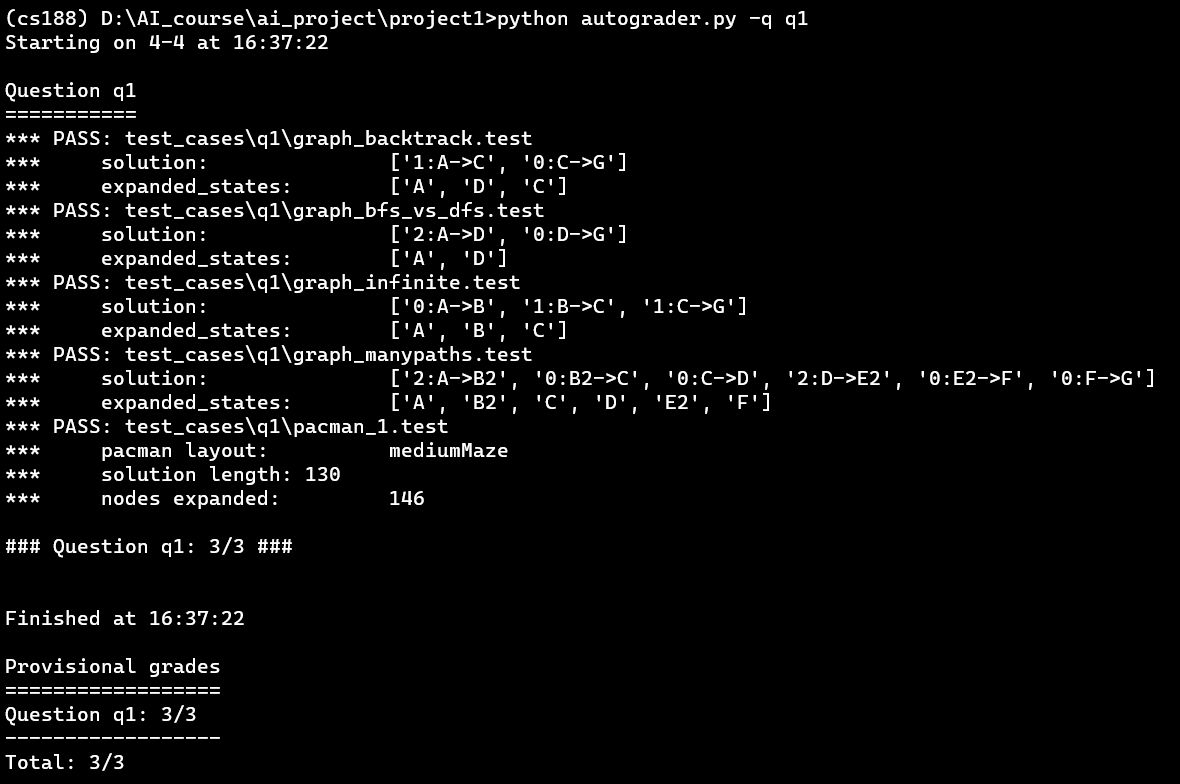
\includegraphics[width=12cm,height=7cm]{1.png}
    \end{figure}

    \normalsize{
        \hspace{1cm}根据上述结果图可以看出在测试$dfs$算法正确性时测试了5个不同的测试用例,
        根据我们编写的$dfs$算法,对于每个测试用例,都会返回对应的解路径以及在这个过程中所扩展
        到的总节点数,并与标准答案进行比对,在测试的最后还会给出测试的得分。\\
    }
    \large{
        \hspace{1cm}\textbf{
            Question 2 (3 points): Breadth First Search\\
        }
    }
    \begin{figure}[h]
        \centering
        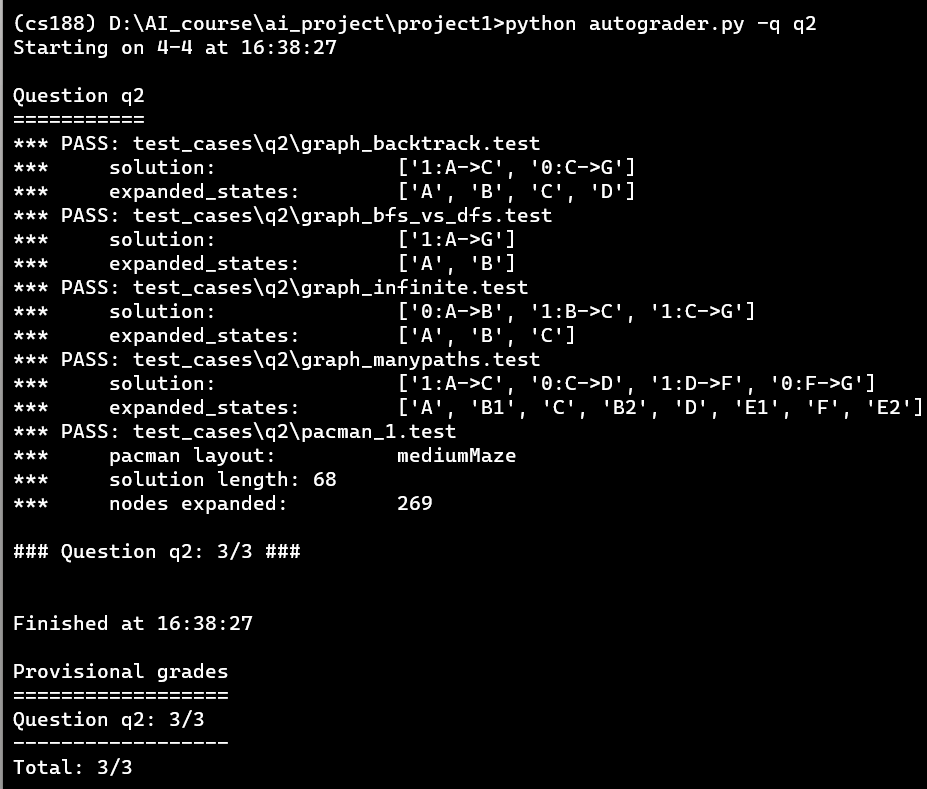
\includegraphics[width=12cm,height=7cm]{2.png}
    \end{figure}
    \normalsize{
        \hspace{1cm}$bfs$的测试用例和$dfs$算法的测试用例一致,只不过在测试程序中将测试算法换为了
        $search.py$文件中的$bfs$算法,虽然两者最终得到的结果是一致的,但从最终返回的解路径以及扩展节点数可以看出
        $bfs$和$dfs$采用了两种不同的搜索策略,应该按需使用。\\
    }
    \large{
        \hspace{1cm}\textbf{
            Question 3 (3 points): Varying the Cost Function\\
        }
    }
    \begin{figure}[h]
        \centering
        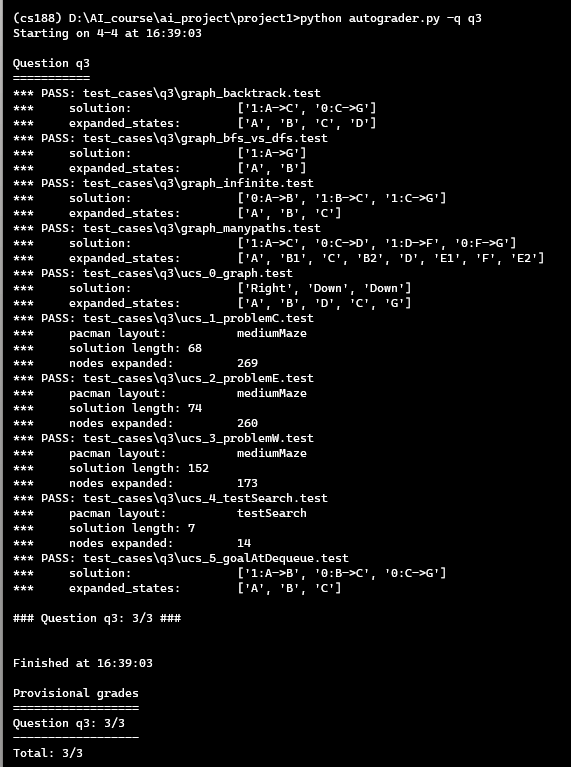
\includegraphics[width=12cm,height=12cm]{3.png}
    \end{figure}
    \normalsize{
        \hspace{1cm}第三个问题是对于$ucs$算法的测试,$ucs$算法,也即是一致代价搜索算法,往往应用于求解最短路径,
        由上图可以看出,针对该算法的测试用例较多,在该测试中,正确的标准不仅仅是返回正确的解路径,还必须符合最短的条件。\\
    }
    \newpage
    \large{
        \hspace{1cm}\textbf{
            Question 4 (3 points): A* search\\
        }
    }
    \begin{figure}[h]
        \centering
        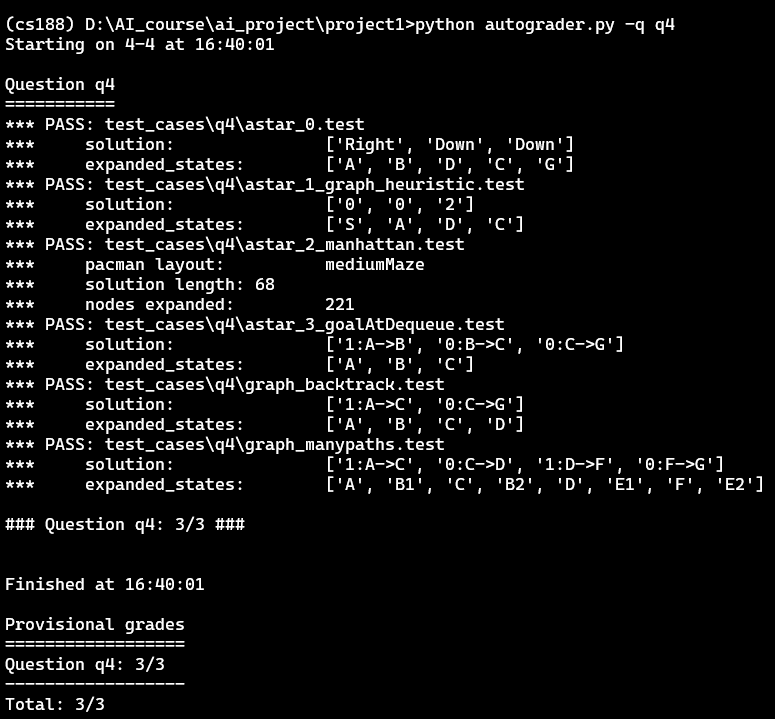
\includegraphics[width=12cm,height=12cm]{4.png}
    \end{figure}
    \normalsize{
        \hspace{1cm}第四个问题是$A*$算法的简单实现,在实现该问题的$A*$算法时,我们只需要对$ucs$算法做出
        简单的改变,将优先队列的优先键值改为启发式函数$f(n)$的值,具体的启发式函数交给之后的子任务完成,测试
        样例中同样是利用$A*$算法去搜索一些固定的迷宫模式,最后返回的结果再次进行检验。\\
    }
    \newpage
    \large{
        \hspace{1cm}\textbf{
            Question 5 (3 points): Finding All the Corners\\
        }
    }
    \begin{figure}[h]
        \centering
        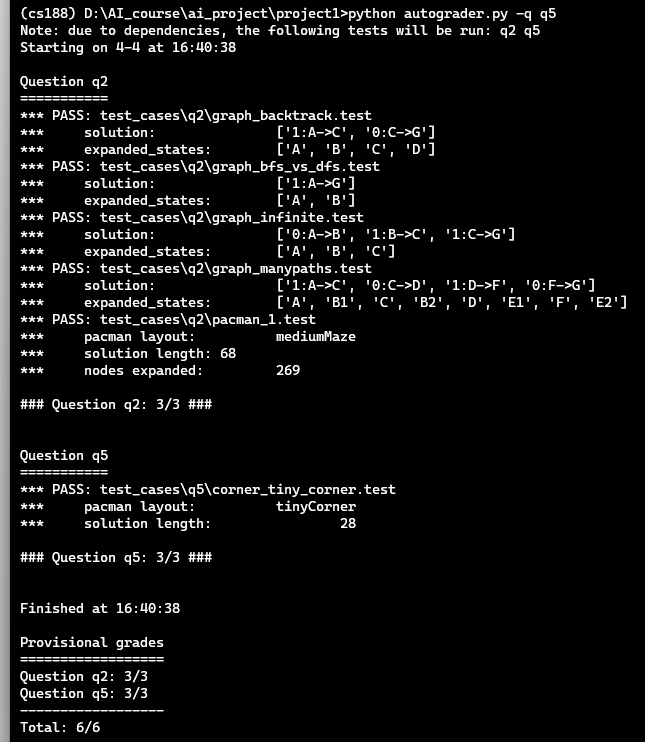
\includegraphics[width=12cm,height=12cm]{5.png}
    \end{figure}
    \normalsize{
        \hspace{1cm}第五个问题以后集中于多目标问题的求解,在本问题中项目主要引导我们模仿之前的类的构造方法
        ,自己补充完成$cornerProblem$类中相应的定义,测试用例同样也发生了改变,会测试我们程序给出的解序列是否能满足
        不重不漏的访问完迷宫的四个角落,并给出具体的扩展路径和长度。\\
    }
    \newpage
    \large{
        \hspace{1cm}\textbf{
            Question 6 (3 points): Corners Problem: Heuristic\\
        }
    }
    \begin{figure}[h]
        \centering
        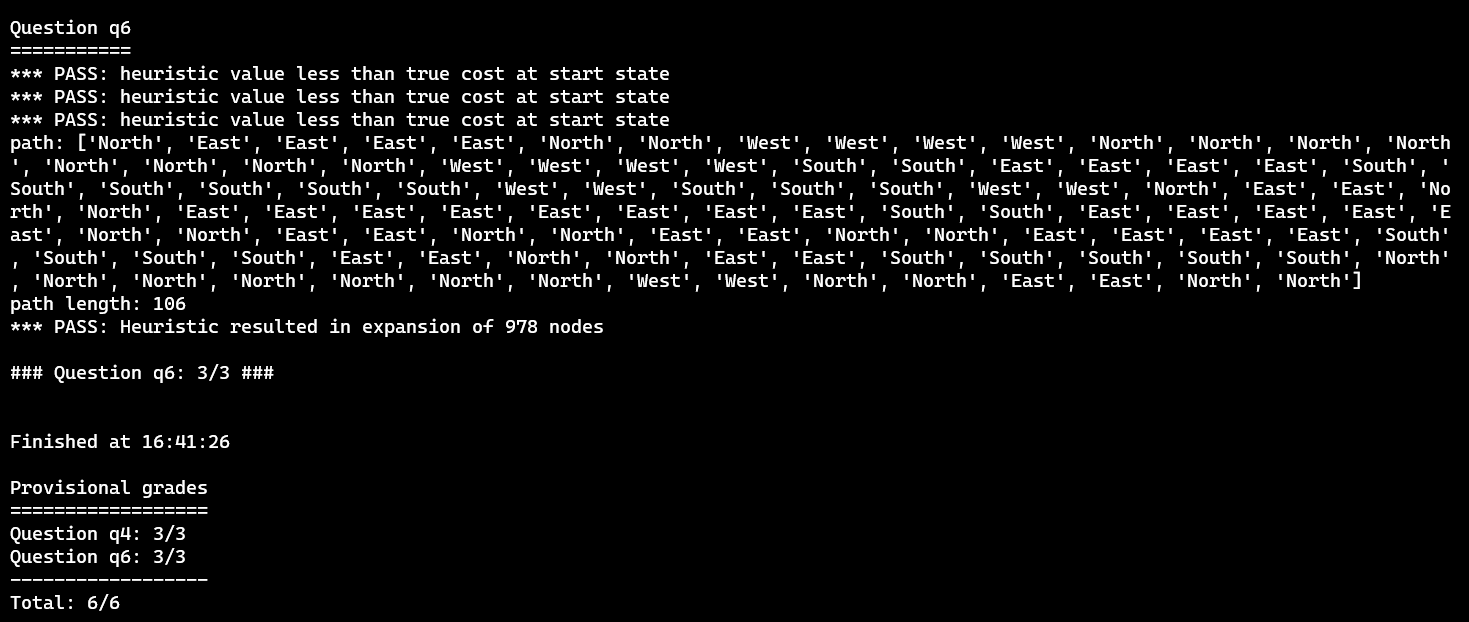
\includegraphics[width=12cm,height=8cm]{6.png}
    \end{figure}
    \normalsize{
        \hspace{1cm}第六个问题考察对于$cornerProblem$中启发式函数的编写,我们按照之前提到的算法思想中的启发式函数设计思路进行
        设计,在测试用例中我们可以看出,该测试程序会首先测试我们编写的启发式函数是否满足一致性和可接受性的要求,其次会测试我们给出
        的解路径是否能够成功的访问到迷宫的四个角落。\\
    }
    \newpage
    \large{
        \hspace{1cm}\textbf{
            Question 7 (4 points): Eating All The Dots\\
        }
    }
    \begin{figure}[h]
        \centering
        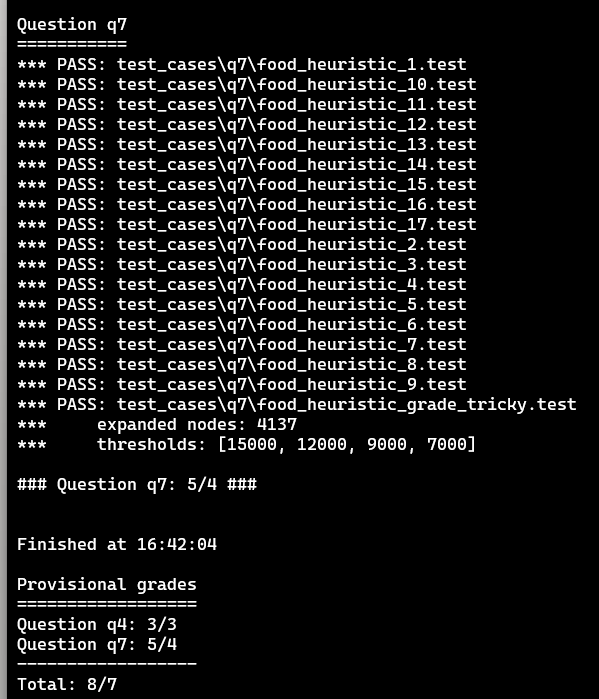
\includegraphics[width=12cm,height=12cm]{7.png}
    \end{figure}
    \normalsize{
        \hspace{1cm}第七个问题中我们对问题做出升级,从固定的寻找迷宫的四个角落的多目标搜索变为迷宫中随机位置的事物的多目标搜索,
        但是我们仍采用第六个问题$cornerProblem$中启发式函数的设计思路进行求解,发现该启发式函数同样可以满足第七个问题的要求,在测试用例中
        我们可以看出测试程序主要是对扩展节点的数目做出了要求,而我们的启发式函数可以满足扩展节点在4000多左右,符合最优要求。\\
    }
    \newpage
    \large{
        \hspace{1cm}\textbf{
            Question 8 (3 points): Suboptimal Search\\
        }
    }
    \begin{figure}[h]
        \centering
        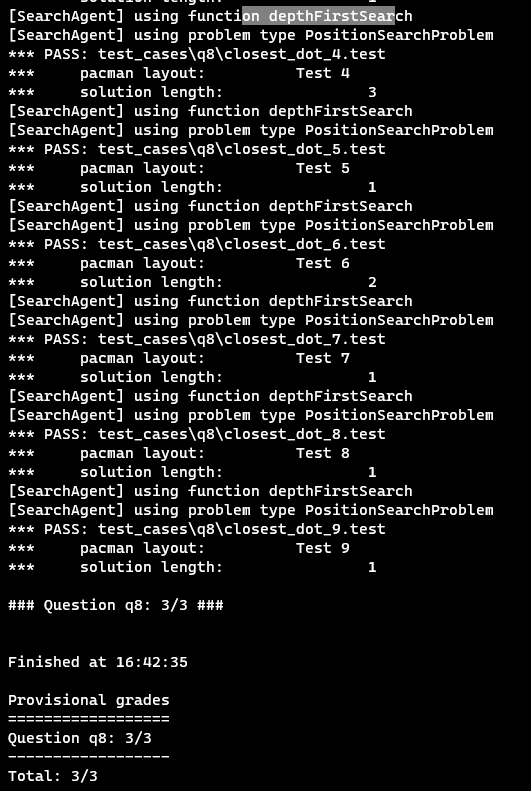
\includegraphics[width=12cm,height=12cm]{8-2.png}
    \end{figure}
    \normalsize{
        \hspace{1cm}第八个问题是简单的应用,我们在理解题意的基础上对原有代码稍加改动并调用
        $ucs$算法求解最近的$food$位置即可解决。\\
    }
    \large{
        \hspace{1cm}\textbf{
           总测试结果如下:\\
        }
    }
    \begin{figure}[h]
        \centering
        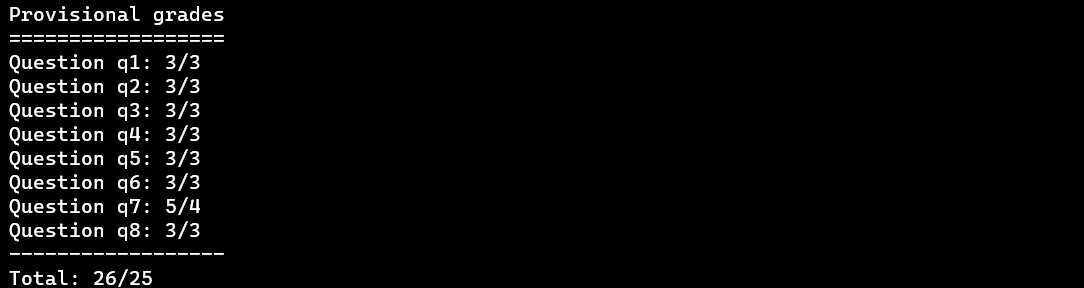
\includegraphics[width=12cm,height=3cm]{9.png}
    \end{figure}
    \newpage
    \Large{
        \textbf{
            五、总结与分析\\
        }
    }
    \large{
        \textbf{
            1、完成项目中遇到的问题\\
        }
    }
    \normalsize{
        \hspace{1cm}(1)在刚开始着手完成本项目时,我的主要问题是找不到从何下手,本项目提供了庞大的基础已有代码,要编写算法以及后续
        的类必须建立在理解整个项目运行原理的前提上,然而我之前对于$python$语言不是很熟悉,一下子接触到如此庞大的$python$代码以及各种
        类的定义时有些无从下手。之后我在仔细阅读项目要求下找出了完成项目所必须理解的几个重要文件,然后开始仔细阅读,遇到不懂的$python$
        用法就结合互联网一起学习,在完成对主要代码的阅读后我对整个项目终于建立起一个基本的认知,明白了一些重要的类的函数,成员变量定义,
        了解了自己编写算法需要使用哪些代码提供的数据结构,需要调用哪些类的函数来帮助自己更好的找到结果。\\
        \hspace{1cm}(2)在找到如何使用已有代码提供的工具后,我顺利完成了前几个子任务(也即是$search.py$中算法的编写),第二次遇到阻碍主要是
        在解决多目标问题搜索的过程中的启发式函数编写,我一开始尝试了许多自己想出的启发式函数,但是都遇到了测试程序返回“该启发式函数不满足
        一致性或可接受性”的要求,在认真理解“一致性与可接受性”的要求后我最终想出以当前节点距离最远的目标节点的距离作为启发式函数的估计值,可以
        证明该距离一定是实际距离的下界且满足“一致性”要求,所以最终完成了启发式函数的编写。\\
    }
    \large{
        \textbf{
            2、本项目中的收获与思考\\
        }
    }
    \normalsize{
        \hspace{1cm}通过该项目的完成,首先我对$python$中的许多基本用法相比之前又有了更深的了解,对于这种大型$python$类搭建构成的
        大型项目也有了更深刻的理解,其次就是有关算法的收获,在本次项目中我自己完成了$python$语言编写的$dfs,bfs,ucs,A*$算法,基本覆盖了
        所有经典的搜索算法,对这些算法有了更深入的了解与认识,在编写这些算法的时候也变的更加熟练,还有最重要的是有关启发式函数的编写,
        通过本项目中多目标搜索的例子,我对$A*$搜索有了更深刻的认识,理解了$A*$算法在人工智能领域的广泛应用,也掌握了有关启发式函数的基本
        要求与编写方法,对于以后编写更加复杂的启发式函数提前做好准备。\\
    }
}
\end{flushleft}
\end{document}

